\documentclass[12pt]{extarticle}
\usepackage{amsmath}
\usepackage{amsfonts}
\usepackage{amssymb}
\usepackage{extsizes}
\usepackage{float}
\usepackage{graphicx}
\usepackage[margin = 1in]{geometry}
\usepackage{hyperref}
\usepackage[english]{babel}
\usepackage[backend=biber, style=numeric]{biblatex}
\usepackage[skins, minted]{tcolorbox}
\usepackage[T1]{fontenc}
\usepackage{lmodern}

\addbibresource{refs.bib}

\usepackage{minted}
\tcbset{listing engine=minted}
\tcbuselibrary{breakable}
\setminted{
	fontsize = \tiny, 
	breaklines,
	linenos = 1,
	numbersep = 2mm,
	autogobble,
	frame = none,
	style = friendly
}

\definecolor{rblue}{HTML}{75AADB}
\definecolor{stanred}{HTML}{B2001D}
\definecolor{jagsyellow}{HTML}{FFCB00}
\newtcbinputlisting{\tcbr}[1]{
	listing file = #1, 
	listing only, 
	minted language = R, 
	title = \lstinline{#1}, 
	minted options = 
	{
		fontsize = \scriptsize, 
		breaklines,
		linenos,
		numbersep = 2mm,
		frame = none,
		style = friendly,
		xleftmargin = 12pt
	}, 
	breakable,
	boxrule = 1pt,
	colback = white,
	colframe = rblue
}
\newtcbinputlisting{\tcbstan}[1]{
	listing file = #1, 
	listing only, 
	minted language = Stan, 
	title = \lstinline{#1}, 
	minted options = 
	{
		fontsize = \scriptsize, 
		breaklines,
		linenos,
		numbersep = 2mm,
		frame = none,
		style = friendly,
		xleftmargin = 12pt
	}, 
	breakable,
	boxrule = 1pt,
	colback = white,
	colframe = stanred
}
\newtcbinputlisting{\tcbjags}[1]{
	listing file = #1, 
	listing only, 
	minted language = R, 
	title = \lstinline{#1}, 
	minted options = 
	{
		fontsize = \scriptsize, 
		breaklines,
		linenos,
		numbersep = 2mm,
		frame = none,
		style = friendly,
		xleftmargin = 12pt
	}, 
	breakable,
	boxrule = 1pt,
	colback = white,
	colframe = jagsyellow
}
\usepackage{lstbayes}
%\usepackage[usenames,dvipsnames]{color}    

\newcommand{\E}{\mathbb{E}}
\newcommand{\Var}{\mathrm{Var}}
\renewcommand{\vec}[1]{\mathbf{#1}}
\newcommand{\Cov}{\mathrm{Cov}}


\begin{document}
	
\title{Bayesian Data Analysis Assignment 2}
\author{Benjamin Cox, S1621312}
\date{\vspace{-5ex}}
\maketitle

\section*{Question 1}

\begin{figure}[H]
	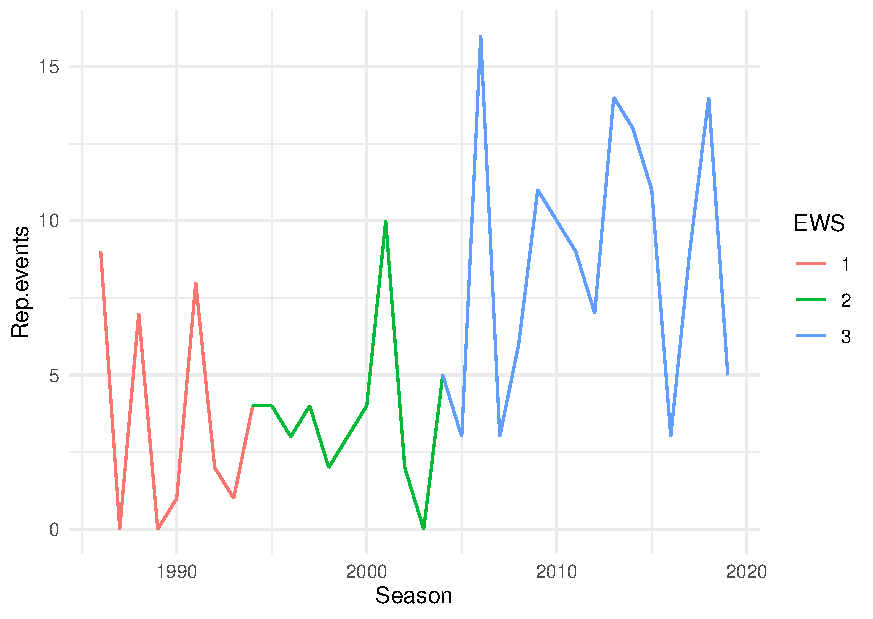
\includegraphics[width = 0.45\textwidth]{../ava_sea}
	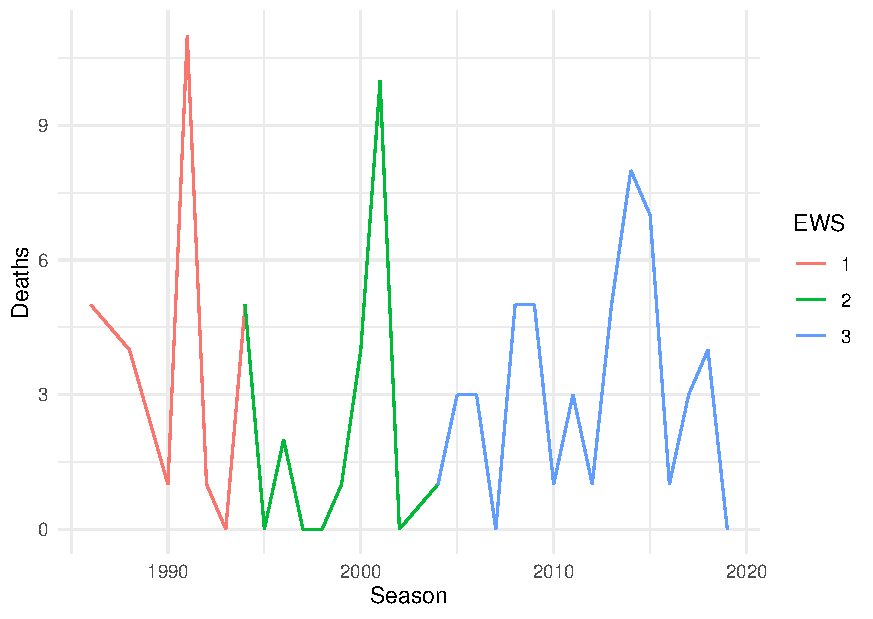
\includegraphics[width = 0.45\textwidth]{../dea_sea}
	\caption{Plots illustrating the temporal evolution of avalanche related statistics. The EWS measure is 1 = No EADS, 2 = EADS extant, 3 = EADS online daily.}
	\label{fig:tempevava}
\end{figure}	

	From the above graphs we can see a broadly positive trend in the number of avalanches and year, but no obvious trend in the number of deaths. We calculate the correlations between the number of deaths and the number of avalanches separated into EWS periods. 
	
	We obtain the following correlations (90\% bootstrap intervals)
\begin{table}[H]
	\centering
	\begin{tabular}{c|c|c}
		\hline
		No EADS & EADS & EADS Online \\
		\hline
		0.807 (0.6397, 0.9986) & 0.875 (0.1890, 0.9728) & 0.602 (0.3842, 0.8147) \\
		\hline
	\end{tabular}
\end{table}
This shows that the events become less correlated after the general public obtained easy access to EADS. It is not likely that the introduction of EADS increased to correlation, so the observed increase in correlation for that period is likely due to noise (10 events in 2001 resulting in 10 deaths). However it may also be due to an increase in user confidence, which led to foolish behaviour.

We are now going to model the number of deaths in avalanches. We are using a Poisson model with a logarithmic (canonical) link function. 

Our formulae are as follows:

\begin{align*}
\lambda_i &= \exp(\beta_0 + \beta_1 \cdot \mathrm{EADS1}_i + \beta_2 \cdot \mathrm{EADS2}_i + \beta_3 \cdot \mathrm{Rep.events}_i)\\
\log(\lambda_i) &= \beta_0 + \beta_1 \cdot \mathrm{EADS1}_i + \beta_2 \cdot \mathrm{EADS2}_i + \beta_3 \cdot \mathrm{Rep.events}_i\\
\mathrm{Deaths}_i &\sim \mathrm{Poisson}(\lambda_i)
\end{align*}

We could model with an offset and without a regression coefficient on the number of avalanches. That model would assume a constant rate per avalanche, which this model does not. We note that this model allows for deaths without an avalanche occurring.

We place wide normal priors on all $\beta_i$ and code up our model. The code is given in \ref{code:stan_1}, with a JAGS version given in \ref{code:jags_1}. 

We are going to run $7$ parallel chains with initial values drawn from a Uniform(-0.1, 0.1) distribution. We are going to run each chain for 3000 iterations and discard the first 1500 (HMC/NUTS converges faster than Gibbs so the length is fine). 

After running we check BGR statistics and find that they have all converged to 1. We also check NUTS specific diagnostics (divergences, energies) and find them satisfactory as well (no divergences, good energy mixing). Therefore we proceed with our analysis.

We obtain the following posterior summaries. We have exponentiated our parameters prior to summarising to ease interpretation.

\begin{table}[ht]
	\centering
\begin{tabular}{r|rrrr}
	\hline
	& (Intercept) $(\beta_0)$ & Rep.events $(\beta_3)$ & EADS1TRUE $(\beta_1)$ & EADS2TRUE $(\beta_2)$\\ 
	\hline
	Min. & 0.35 & 1.09 & 0.22 & 0.12 \\ 
	1st Qu. & 0.86 & 1.19 & 0.71 & 0.32 \\ 
	Median & 1.05 & 1.22 & 0.88 & 0.39 \\ 
	Mean & 1.08 & 1.22 & 0.92 & 0.41 \\ 
	3rd Qu. & 1.26 & 1.24 & 1.08 & 0.48 \\ 
	Max. & 2.62 & 1.38 & 3.01 & 1.32 \\ 
	\hline
\end{tabular}
\caption{Posterior summaries for the first Poisson model}
\label{tab:postsum_po}
\end{table}

From this we can make some initial conclusions. We see that the expected number of deaths per year given no mitigation (ie all other covariates 0) is 1.08. We also see that each EADS evolution decreases the expected number of deaths, by 0.92 and 0.41 times respectively (if all other variables are held constant). The latter is a rather large decrease, befitting of the drastic change in preparation tact that the EADS going online brought about. We also see that each avalanche increases the number of expected deaths 1.22 times. This means that avalanches get exponentially more dangerous the more that there are, which seems somewhat strange.

We are interested in the posterior predictive distribution. We want to predict the probability of observing less than 15 deaths given 20 avalanches next year. We know that the EADS will still be online, so we have the appropriate data. 

We obtain a probability of $P(\mathrm{Deaths}<15|\mathrm{Rep.events}=20, \mathrm{EADS}=2) = 0.185$ with a 95\% bootstrap interval of $(0.1838, 0.1864)$. This is rather low, but this is expected given that large number of avalanches (and that they get more dangerous the more there are.)

We are also interested in the probability of observing more than 1 death in mean per avalanche in each stage of the EADS lifespan (not present, present, online). For this we need to calculate $$P\left(\frac{\lambda}{\mathrm{Rep.events}}>1 \ \vline \ \mathrm{EADS}=x\right).$$ Given our offsetting this is rather simple, as this simplifies to $$P\left(\exp(\beta_0 + \beta_1 \cdot \mathrm{EADS1} + \beta_2 \cdot \mathrm{EADS2}) > 1 | \mathrm{EADS} = x\right),$$
of which we have posterior samples.

We calculate these probabilities for all values of the EADS and obtain
\begin{table}[ht]
	\centering
\begin{tabular}{ccc}
	\hline
	No EADS & EADS & EADS online \\
	\hline
	0.105 & 0.005 & 0 (machine precision) \\
	\hline
\end{tabular}
\caption{Probabilities of multiple fatalities per avalanche given the various states of the EADS}
\label{tab:probmdpa}
\end{table}

After this we are told that on average the number of avalanches per year is between 5 and 15, and that they consider that for an extreme number of events that the number of casualties could be 4 times greater (or lesser) than the average number of casualties. 

From this we work out that the mean number of avalanches is 10 with standard deviation 5. We also want to give the multiplier high mass between 0.25 and 4. 

Suggested is a log-normal prior with mean 0 and standard deviation 2 on $\phi = \exp((x-\mu_x)\cdot\beta_{\mathrm{Rep.events}}),$ the multiplier. This implies a normal prior with mean 0 and standard deviation 2 for $(x-\mu_x)\cdot\beta_{\mathrm{Rep.events}}$, or $\beta_{\mathrm{Rep.events}} \sim N(\mu = 0, \sigma^2 = 4(x-\mu_x)^2).$ There could be problems with this, as it is possible for $(x-\mu_x)$ to be 0. 

The mean and standard deviation parameters for a lognormal distribution are typically given as the mean and standard deviation of the underlying normal distribution. Hence we calculate the true mean and SD as \[\mu_{\phi} = \exp\left(0 + \frac{2^2}{2}\right) = e^2 \approx 7.39, \qquad \sigma^2_{\phi} = (\exp(2^2)-1)\exp(2\cdot0 + 2^2) = e^8 - e^4 \approx 2925, \implies \sigma \approx 54.\] This is clearly not appropriate for the multiplier, as the mean is too high, and the standard deviation even moreso.

We are now going to expand our model to include a term to capture randomness not accounted for by the other components. We are going to design the model as follows

\begin{align*}
\theta_{hyp} &\sim \mathrm{Uniform}(0, 10),\\
\theta &\sim \mathrm{Normal}(0, \theta_{hyp}),\\
\lambda_i &= \exp(\beta_1 \cdot \mathrm{EADS1}_i + \beta_2 \cdot \mathrm{EADS2}_i + \beta_3 \cdot \mathrm{Rep.events}_i + \theta)\\
\log(\lambda_i) &= \beta_1 \cdot \mathrm{EADS1}_i + \beta_2 \cdot \mathrm{EADS2}_i + \beta_3 \cdot \mathrm{Rep.events}_i + \theta\\
\mathrm{Deaths}_i &\sim \mathrm{Poisson}(\lambda_i)
\end{align*} 

This model is a lot more computationally complex than the other model and requires us to make some tweaks to the sampling and model code in order to make it converge well. It runs significantly slower than the previous model, but we do get convergence. We have re-parametrised and de-centred the model so that it is mathematically equivalent, but we are dealing with standard normals and multiples thereof, rather than working with normals with variable $\sigma$. 

To make this model run well we must remove the intercept term. This is because $\theta$ and the intercept term serve the same purpose; capture the latent effect. Therefore the intercept term must be removed, as $\theta + \beta_0$ should be constant, but this does not constrain either of them, thus without removing the intercept we do not get convergence. We note that $\beta_0$ had a normal prior with mean 0, so $\theta$ should well compensate for it.

We are going to run $4$ parallel chains with initial values drawn from a Uniform(-0.05, 0.05) distribution. We are going to run each chain for 8000 iterations and discard the first 4000 (HMC/NUTS converges faster than Gibbs so the length is fine). We are going to increase the maximum tree depth to 15 (from 10) and increase the adaptation acceptance probability to 0.99 (from 0.8). These will help us to deal with the implied distributional shape given by the uniform-normal combination. It will significantly slow sampling, but this is required for convergence.

After running we check BGR statistics and find that they have all converged to 1. We also check NUTS specific diagnostics (divergences, energies) and find them satisfactory as well (no divergences, good energy mixing). Therefore we proceed with our analysis.

This is one of the few times I have seen JAGS converge better than Stan, as the NUTS sampler finds it somewhat tricky to deal with the implied distribution space given by the normal-uniform combination alongside the others. We have to run for more iterations and with a smaller stepping than we would like, so it takes significantly longer to run. A single chain of this model takes over 3 times as long as all of the chains of the previous model. Given all of this it should give us a lot better predictions right?

Well, no.

We obtain the following table for our posterior values

\begin{table}[ht]
	\centering
	\begin{tabular}{r|rrrr}
		\hline
		& Rep.events $\exp(\beta_3)$ & EADS1TRUE $\exp(\beta_1)$ & EADS2TRUE $\exp(\beta_2)$ & theta $\exp$($\theta$) \\ 
		\hline
		Min. & 1.09 & 0.26 & 0.12 & 0.37 \\ 
		1st Qu. & 1.19 & 0.73 & 0.32 & 0.89 \\ 
		Median & 1.22 & 0.89 & 0.40 & 1.02 \\ 
		Mean & 1.22 & 0.93 & 0.42 & 1.06 \\ 
		3rd Qu. & 1.24 & 1.08 & 0.49 & 1.21 \\ 
		Max. & 1.36 & 2.99 & 1.34 & 3.35 \\ 
		\hline
	\end{tabular}
\caption{Posterior summaries for the second Poisson model, which attempts to encapsulate the extra variability.}
\label{tab:postsum_poexv}
\end{table}

Observe that these are mostly the same as the estimates that we got above, with the exception that we have $\theta$ rather than $\beta_0$. However $\theta$ has different distributional properties not captured in this table that make it somewhat better for this task. 

Now we are going to compare the two models and make some recommendations. Comparing the posterior predictives for the data they give identical results: 

\begin{figure}[H]
	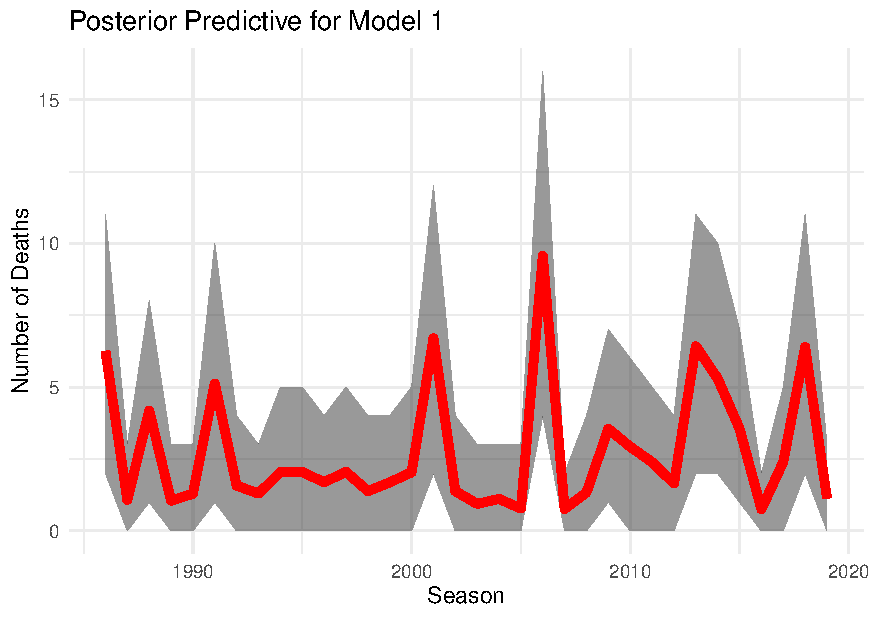
\includegraphics[width = 0.45\textwidth]{../ppmod1}
	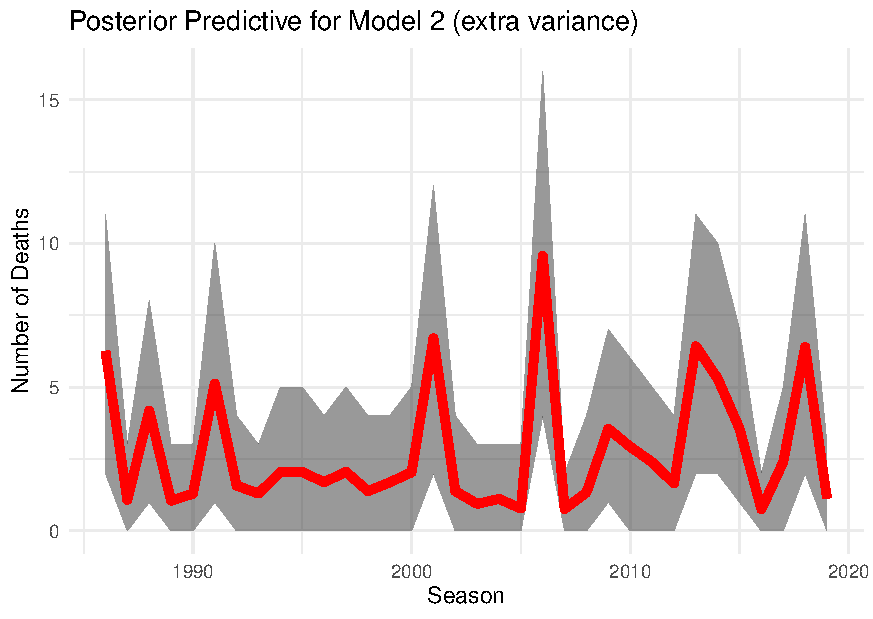
\includegraphics[width = 0.45\textwidth]{../ppmod2}
	\caption{Posterior predictive plots for the data. Note that they are identical. the red line indicates the predictive mean, and the bands indicate the 90\% credible interval.}
	\label{fig:postpreddata}
\end{figure}

Comparing the parameter summaries tells a similar story: 

\begin{figure}[H]
	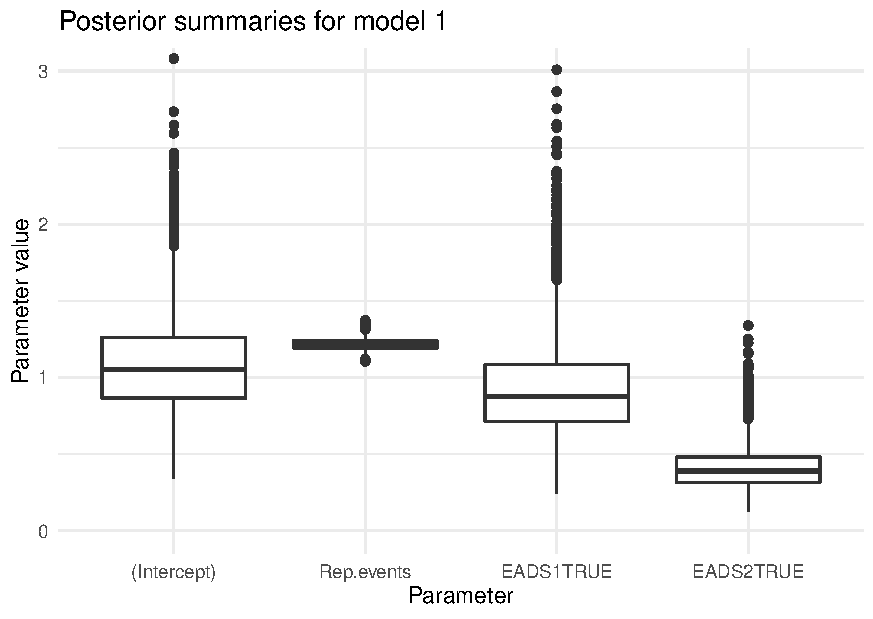
\includegraphics[width = 0.45\textwidth]{../psmod1}
	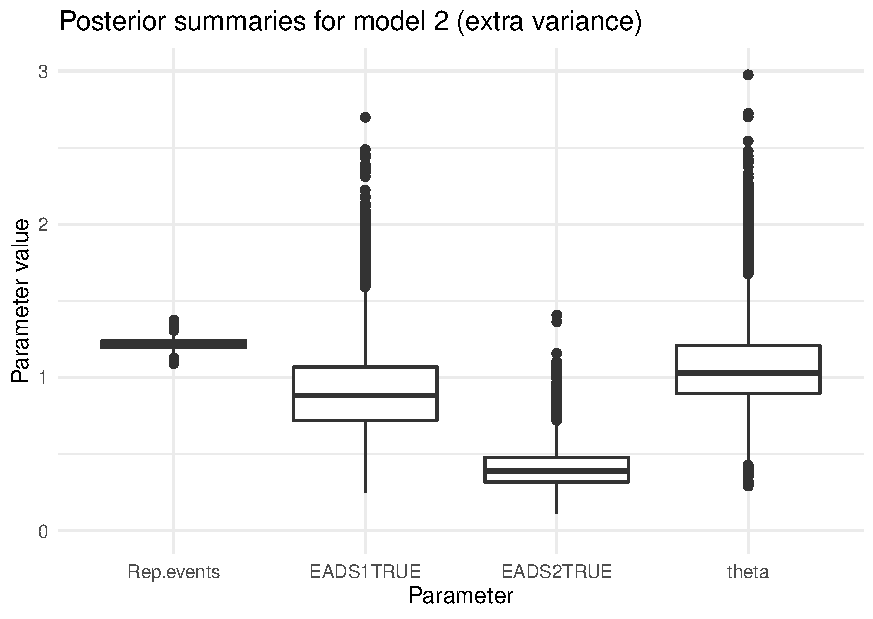
\includegraphics[width = 0.45\textwidth]{../psmod2}
	\caption{Posterior summaries for the parameters for each model. The parameters have been exponentiated to ease interpretation.}
	\label{fig:postsummods}
\end{figure}
We see that there is more variability in theta than in the intercept, but both models will lead to the same conclusions as they are very similar in terms of distribution. 

Calculating the Deviance Information Criterion for both models we get a DIC of 141.9 for the first model and a DIC of 141.6 for the second. Based on this we would weakly prefer the second model, as it has a smaller DIC. 

However I would prefer the first model. The DICs are very similar in size, and given the stochastic nature overlap distributionally quite a bit. However the first model is both more interpretable and more stable. The first model converges better and samples faster. Both lead to the same conclusions, so I don't see much reason to choose the second. 

However I propose a third model. I believe that a model of the first form with the number of avalanches as an offset rather than as a covariate makes the most sense. This is because it would mean that each avalanche is not inherently more dangerous than the last. It would also ease interpretation further, as the calculated rates would be deaths per avalanche. Furthermore it would eliminate the predictions of deaths without avalanches occurring, which is a problem with the two previous models. 

However it would not account for some years having more avalanches and thus being more dangerous than other years. I believe that this model makes more sense (and believed that it was the model we were being asked to work on prior to corresponding with the lecturer), but the biggest weakness is what I just mentioned. This model is more classical Poisson, but does not allow for some more advanced deductions. 

\section*{Question 2}

We have data on each avalanche reported in the Piedmont region between 2014 and 2019. The data contains the year reported (Season), the number of people involved (Hit), the number of fatalities (Deaths), and the nearest recording station (Rec.station). Furthermore for each recording station the total amount of snow (Snow\_total, cm) and the snow permanence (Snow\_days, days) are recorded for each year. The recording stations are divided into 3 geographical regions (Geo.space). 

We transform Snow\_days into Snow\_fnights by dividing by 14. This gives us the permanence in fortnights. We transform Snow\_total into Snow\_meters by dividing by 100. This gives us the amount of snow in meters.  We do not round, as this would lose information. 

We mean-centre both Snow\_fnights and Snow\_meters, as they are continuous variables, so centering them will both aid in interpretation and in sampler convergence. 

We subtract the minimum of Season from Season, meaning that we interpret Season as the number of years since 2014. This will aid in interpretation and in sampler convergence. 

None of these transformations will change correlations or variance, as they are additive. 

We obtain the following correlations between our three variables. 
\begin{table}[ht]
	\centering
	\begin{tabular}{r|rrr}
	Pearson Correlation	& Season & Snow\_meters & Snow\_fnights \\ 
		\hline
		Season & 1.00 & -0.10 & -0.10 \\ 
		Snow\_meters & -0.10 & 1.00 & 0.83 \\ 
		Snow\_fnights & -0.10 & 0.83 & 1.00 \\ 
	\end{tabular}
\end{table}

From this we can deduce a weak negative correlation between Season and both Snow\_meters and Snow\_fnights, likely due to climate change. Furthermore we see that Snow\_meters and Snow\_fnights are extremely highly correlated, as expected (more snow means more time for snow to melt). This could prove to be a problem, so we will address this later. 

We are interested in fitting a random effects model for the proportion of fatalities in an avalanche. We assume fixed effects for Season, Snow\_meters,and Snow\_fnights, with a random effect on Geo.space. This is characterised by the following equations:

\begin{align*}
\mathrm{logit}(p_i) &= \beta_1 \cdot \mathrm{Season} + \beta_2 \cdot \mathrm{Snow\_meters} + \beta_3 \cdot \mathrm{Snow\_fnight} + R_{\mathrm{Geo.space}_i}\\
R_i \equiv R_{\mathrm{Geo.space}_i} &\sim \mathrm{Normal}(0, R_{hyp})\\
R_{hyp} &\sim \mathrm{Uniform}(0, 10)\\
\beta_i &\sim \mathrm{Normal}(0, 10)\\
\mathrm{Deaths}_i &\sim \mathrm{Binomial}(\mathrm{Hit}_i, p_i)
\end{align*}

Note that there is no intercept as the random effects on the geographical location serve the same purpose. If we included an intercept we would not get repeatable results as the random effects would be offset by the intercept, thus both the intercept and random effects would converge to different values in each run (but would sum to the same distribution). We would include an intercept if some events had no random effect associated, but that is not the case here.

We are going to run $4$ parallel chains with initial values drawn from a Uniform(-0.1, 0.1) distribution. We are going to run each chain for 10000 iterations and discard the first 5000 (HMC/NUTS converges faster than Gibbs so the length is fine). We are going to increase the adaptation acceptance probability to 0.95 (from 0.8). These will help us to deal with the implied distributional shape given by the uniform-normal combination. It will significantly slow sampling, but this is required for convergence. We have implemented this model in both Stan and JAGS, but we will use the Stan samples for this analysis (both of them agree on the summaries anyway.) The Stan code is in \ref{code:stan_2} with the main R script in \ref{code:main_2}, whereas the JAGS code and R script is in \ref{code:jags_2}. All the code for this question is contained in these categories.

After running we check BGR statistics and find that they have all converged to 1. We also check NUTS specific diagnostics (divergences, energies) and find them satisfactory as well (no divergences, good energy mixing). Therefore we proceed with our analysis.

We obtain the following posterior summaries for our parameters:

\begin{table}[ht]
	\centering
	\footnotesize
	\begin{tabular}{r|rrrrrr}
		\hline
		& Season ($\beta_1$) & Snow\_meters ($\beta_2$) & Snow\_fnights ($\beta_3$) & Geo\_space1 ($\mathrm{R}_{1}$) & Geo\_space2 ($\mathrm{R}_{2}$) & Geo\_space3 ($\mathrm{R}_{3}$)\\ 
		\hline
		Min. & -0.69 & -1.01 & -0.71 & -2.12 & -1.70 & -3.89 \\ 
		1st Qu. & -0.27 & -0.33 & -0.04 & -0.09 & -0.26 & -0.87 \\ 
		Median & -0.19 & -0.19 & 0.08 & 0.10 & -0.05 & -0.40 \\ 
		Mean & -0.18 & -0.18 & 0.08 & 0.18 & -0.07 & -0.52 \\ 
		3rd Qu. & -0.10 & -0.04 & 0.19 & 0.45 & 0.11 & -0.07 \\ 
		Max. & 0.43 & 0.89 & 0.80 & 2.83 & 1.36 & 1.24 \\ 
		\hline
	\end{tabular}
\caption{Posterior summaries for the first binomial random effects model, which has the effects on geographical area}
\label{tab:postsum_binmod1}
\end{table}

These parameters have an effect on the logit scale, meaning that they affect the log-odds of deaths:survived. For example a snow depth of 1 meter above the mean subtracts 0.18 from the expected log-odds (all other variables held constant). This means that survival becomes more likely the more snow that has occurred. 

Looking at the regions we see that region 1 is more dangerous than region 2, which is more dangerous than region 3 (if all other variables are the same). 

Some of these estimates seem strange, as we would intuitively think that more snow is more deadly. The seasonal trend is expected, and the geographical trend is interesting. However the high correlation between the amount of snow and its permanence seems to be affecting the model, as realistically both of them should have the same sign due to their correlation. Therefore we propose a second model without the Snow\_fnights term.

\[
\mathrm{logit}(p_i) = \beta_1 \cdot \mathrm{Season} + \beta_2 \cdot \mathrm{Snow\_meters} + R_{\mathrm{Geo.space}_i}
\]

We perform the same adjustments to the sampler that we did for this model, and check the same statistics.

We obtain the following posterior summaries for our parameters:

\begin{table}[ht]
	\centering
	\begin{tabular}{r|rrrrr}
		\hline
		& Season ($\beta_1$) & Snow\_meters ($\beta_2$) & Geo\_space1 ($\mathrm{R}_{1}$) & Geo\_space2 ($\mathrm{R}_{2}$) & Geo\_space3 ($\mathrm{R}_{3}$)\\ 
		\hline
		Min. & -0.87 & -0.56 & -2.04 & -1.51 & -3.12 \\ 
		1st Qu. & -0.26 & -0.17 & -0.10 & -0.24 & -0.93 \\ 
		Median & -0.18 & -0.09 & 0.13 & -0.03 & -0.57 \\ 
		Mean & -0.18 & -0.10 & 0.20 & -0.05 & -0.61 \\ 
		3rd Qu. & -0.09 & -0.02 & 0.50 & 0.14 & -0.23 \\ 
		Max. & 0.35 & 0.29 & 2.91 & 1.73 & 0.72 \\ 
		\hline
	\end{tabular}
\caption{Posterior summaries for the second binomial random effects model, which has the effects on geographical area. This model has been adjusted to compensate for collinearity between Snow\_meters and Snow\_fnights.}
\label{tab:postsum_binmod2}
\end{table}

Looking at the tables we come to very similar conclusions. Of particular note is that $\beta_2$ has mean equal to the sum of the means of the previous $\beta_2$ and $\beta_3$. This is due to the high correlation between these variables. 

This means that the random effects are more prominent. Notable is that the 3rd region seems more dangerous under this model. 

We are now interested in the posterior distribution for the proportion of deaths expected at stations 1, 8, and 10 for the 2015 and 2018 seasons. We obtain the following means and 95\% credible intervals:

\begin{table}[ht]
	\centering
	\begin{tabular}{r|rr|rr|rr}
			\hline
			& Station 1: 2015 & 2018 & Station 8: 2015 & 2018 & Station 10: 2015 & 2018 \\
			\hline
			Mean & 0.45 & 0.33 & 0.51 & 0.31 & 0.37 & 0.23 \\
			Interval & (0.24, 0.69) & (0.12, 0.63) & (0.34, 0.65) & (0.14, 0.51) & (0.19, 0.54) & (0.09, 0.41)\\
			\hline
	\end{tabular}
\caption{Posterior summaries for the predicted proportion of casualties near the given recording stations in the given years. Data from the years has been used to construct these statistics.}
\label{tab:postprop}
\end{table}

We are also interested in comparing the probabilities of having a proportion of deaths greater than 60\% between the stations. We obtain the following table:

\begin{table}[ht]
	\centering
	\begin{tabular}{l|r|r|r}
		\hline
		Year & Station 1 & Station 8 & Station 10 \\
		\hline
		2015 & 0.10 & 0.08 & 0.003 \\
		2018 & 0.04 & 0.003 & 0.00 \\
		\hline
	\end{tabular}
	\caption{Posterior probabilities of having a proportion of deaths greater than 60\% near these stations in the years of interest.}
	\label{tab:post_60}
\end{table}

After the success of this model we might be interested in fitting a model with more granular random effects. Therefore we propose a model with a random effect on the station, not on the geographical area. We will design the model with the following formula:

\begin{align*}
\mathrm{logit}(p_i) &= \beta_1 \cdot \mathrm{Season} + \beta_2 \cdot \mathrm{Snow\_meters} + \beta_3 \cdot \mathrm{Snow\_fnight} + R_{\mathrm{Station}_i}\\
R_i \equiv R_{\mathrm{Station}_i} &\sim \mathrm{Normal}(0, R_{hyp})\\
R_{hyp} &\sim \mathrm{Uniform}(0, 10)\\
\beta_i &\sim \mathrm{Normal}(0, 10)\\
\mathrm{Deaths}_i &\sim \mathrm{Binomial}(\mathrm{Hit}_i, p_i)
\end{align*}
This model is very similar to our previous model, but we expect more finely tuned results. We will also be able to assess the relative danger of stations (somewhat). 

We run the sampler with the same settings as above and obtain the following summary statistics: 

\begin{table}[H]
	\centering
	\begin{tabular}{r|rrrrrrr}
		\hline
		& Season & Snow\_meters & Rec.station1 & Rec.station2 & Rec.station3 & Rec.station4 & Rec.station5 \\ 
		\hline
		Min. & -0.77 & -0.97 & -1.62 & -16.32 & -6.27 & -6.44 & -2.74 \\ 
		1st Qu. & -0.30 & -0.23 & 0.77 & -1.22 & -1.12 & -1.64 & -0.05 \\ 
		Median & -0.21 & -0.11 & 1.55 & -0.37 & -0.50 & -1.03 & 0.33 \\ 
		Mean & -0.21 & -0.12 & 1.78 & -0.59 & -0.60 & -1.12 & 0.36 \\ 
		3rd Qu. & -0.12 & 0.00 & 2.50 & 0.23 & 0.00 & -0.48 & 0.75 \\ 
		Max. & 0.31 & 0.56 & 14.07 & 6.94 & 3.05 & 1.49 & 3.33 \\ 
		\hline
	\end{tabular}

\vspace{1em}

	\begin{tabular}{r|rrrrrr}
		\hline
		& Rec.station6 & Rec.station7 & Rec.station8 & Rec.station9 & Rec.station10 & Rec.station11 \\ 
		\hline
		Min. & -6.73 & -5.21 & -1.92 & -4.96 & -4.33 & -3.63 \\ 
		1st Qu. & -1.25 & 0.05 & -0.01 & -1.60 & -0.69 & -0.74 \\ 
		Median & -0.62 & 0.72 & 0.33 & -1.04 & -0.16 & -0.29 \\ 
		Mean & -0.72 & 0.96 & 0.35 & -1.11 & -0.20 & -0.32 \\ 
		3rd Qu. & -0.09 & 1.65 & 0.70 & -0.53 & 0.31 & 0.10 \\ 
		Max. & 2.63 & 18.10 & 3.29 & 1.70 & 3.54 & 2.58 \\ 
		\hline
	\end{tabular}
\caption{Posterior summaries for the third binomial random effects model, which has the effects on the recording station. This model has been adjusted to compensate for collinearity between Snow\_meters and Snow\_fnights.}
\label{tab:postsum_binmod3}
\end{table}

We also obtain the following means and 95\% credible intervals for the proportion of casualties near the given stations in the given years. 

\begin{table}[H]
	\centering
	\begin{tabular}{r|rr|rr|rr}
		\hline
		& Station 1: 2015 & 2018 & Station 8: 2015 & 2018 & Station 10: 2015 & 2018 \\
		\hline
		Mean & 0.72 & 0.61 & 0.58 & 0.37 & 0.47 & 0.30 \\
		Interval & (0.34, 0.99) & (0.18, 0.98) & (0.12, 0.68) & (0.14, 0.51) & (0.15, 0.79) & (0.06, 0.66)\\
		\hline
	\end{tabular}
	\caption{Posterior summaries for the predicted proportion of casualties near the given recording stations in the given years. Data from the years has been used to construct these statistics. This model has the random effect on the station, not geographical area as previous.}
	\label{tab:postprop_stat}
\end{table}

These have much wider credible intervals, reflecting the relative lack of data that we have for each station. This model does not take into account geographical similarity between stations which lead to similar casualty proportions. We also often have only one point of data per station per year, leading to the estimates being overfit to the data. We have 43 data points and 13 parameters. 

I would be inclined to say that we are overfitting on the station level, thus we should incorporate variability from the geographical level as well. This will add more parameters, but they will be more constrained on each other rather than biased on the data.

Comparing the two models above using the DIC we obtain a DIC of 91.04 for the model with effects on geographical area and a DIC of 85.21 for the model with effects of the nearest station. This is due to the better fit: the penalty terms are 4.171 and 8.854 respectively, showing the effect of the increased number of parameters. Based on this we would prefer the station level model. However both of them lead to similar conclusions.

We could have a random effect on the recording station drawn from the geographical area drawn from an overarching distribution. We propose the following model:

\begin{align*}
\sigma_1, \sigma_2 &\sim \Gamma(1, 0.1), \\
\mu_{\mathrm{Geo.space}_i} &\sim \mathrm{Normal}(0, \sigma_2^{-2})\\\
R_{\mathrm{(Rep.station, Geo.space)}_i} &\sim \mathrm{Normal}(\mu_{\mathrm{Geo.space}_i}, \sigma_1^{-2}),\\
\mathrm{logit}(p_i) &= \beta_1 \cdot \mathrm{Season} + \beta_2 \cdot \mathrm{Snow\_meters} + R_{\mathrm{(Rep.station, Geo.space)}_i}, \\
\mathrm{Deaths}_i &\sim \mathrm{Binomial}(\mathrm{Hit}_i, p_i),
\end{align*}

which we have encoded in JAGS in \texttt{binom\_doublereff.jags}. This model works rather well. It has a DIC of 86.82, which is slightly higher than that of the station level model, but more than compensates for it in the information that we can glean from it, as we can observe both geographical and station level effects, rather than just station level. 
\printbibliography

\newpage

\appendix

\section{Code for Question 1}
\subsection{R}
%\inputminted{R}{../Q1.R}
\tcbr{../Q1.R}
\label{code:main_1}
\subsection{Stan}
\tcbstan{../stan/poisson_glm.stan}
\tcbstan{../stan/poisson_glm_exvar.stan}
\label{code:stan_1}
\subsection{JAGS}
\tcbr{../jags/Q1jags.R}
\tcbjags{../jags/poisson.jags}
\tcbjags{../jags/poisson_exvar.jags}
\label{code:jags_1}
\section{Code for Question 2}
\subsection{R}
\tcbr{../Q2.R}
\label{code:main_2}
\subsection{Stan}
\tcbstan{../stan/binomial_glm.stan}
\tcbstan{../stan/binomial_glm_randomeffects.stan}
\label{code:stan_2}
\subsection{JAGS}
\tcbr{../jags/Q2jags.R}
\tcbjags{../jags/binom_reff.jags}
\tcbjags{../jags/binom_reff_nofn.jags}
\tcbjags{../jags/binom_doublereff.jags}
\label{code:jags_2}
\end{document}

